\chapter{Method}\label{chap:method}
\label{sec:second}
\section{The naive subsampler}\label{subsec:naive}
The most intuitive and naive method to reduce the computational cost of a Metropolis-Hastings sampler, in terms of subsampling, is to randomly choose a subset of the data at each iteration, and calculate the log-likelihood ratio. In other words, step 5 in Algorithm \ref{algo:MH} is calculated for the selected subset only. We call this method the naive subsampler.  However, as is pointed out by \cite{Bardenet:1}, this method does not have the correct posterior distribution as its invariant distribution. Instead the invariant distribution of the naive subsampler is a broadened version of the posterior, due to large variance in the log-likelihood ratio. 
 \section{Firefly Monte Carlo}\label{sec:Firefly}
In their paper from 2014, Maclaurin and Adams  introduced the Firefly Monte Carlo method \cite{Maclaurin:1}. 
The aim of this method is to reduce the computational cost of MH-like algorithms by evaluating the likelihood function for only a subset of the data, while still keeping the true full-data posterior distribution as the invariant distribution of the Markov chain. As we will see, this is a method with similarities to the naive subsampler, but with some changes in order to preserve the correct invariant distribution.  \\ \\
We assume the data $x_n$ are conditionally independent given $\theta$.
For each data point $x_n$ Maclaurin and Adams introduce an auxiliary variable $z_n \in \{0, 1\}$, and they make use of a strictly positive lower bound, $B_n\left(\theta\right)$ of the likelihood of the $n$'th data point, $L_n\left(\theta\right)$, meaning that the condition 
\begin{equation}
    B_n\left(\theta\right) \leq L_n\left(\theta\right)
\end{equation} is met for all $\theta$ and all $n$. 
The $z_n$'s are  Bernoulli distributed, conditioned on the parameters $x_n$ and $\theta$, 
and drawn from the  Bernoulli distribution:
\begin{equation}\label{eq:auxiliary_dist}
    p(z_n\mid x_n,\theta) = \left[\frac{L_n(\theta) - B_n(\theta)}{L_n(\theta)}\right]^{z_n}\left[\frac{B_n(\theta)}{L_n(\theta)}\right]^{1-z_n} \quad .
\end{equation}
We say that a data point $x_n$ is bright if $z_n = 1$, and that it is dark if $z_n = 0$. 
From \eqref{eq:auxiliary_dist}, we see that a data point $x_n$ is more likely to be dark if $L_n(\theta) - B_n(\theta)$ is small, i.e. the lower bound $B_n(\theta)$ is tight to the likelihood $L_n(\theta)$. Including these auxiliary variables, we get the following joint probability distribution. 
\begin{equation*}
\begin{split}
     p(\theta, \{z_n\}_{n=1}^N\mid\{x_n\}_{n=1}^N) &\propto p(\theta, \{x_n, z_n\}_{n = 1}^N) \\
     &= p(\theta) p(\{x_n, z_n\}_{n=1}^N\mid\theta) \\
     & = p(\theta)p(\{x_n\}_{n=1}^N\mid\theta)p(\{z_n\}_{n=1}^N\mid \{x_n\}_{n=1}^N, \theta)
\end{split}
\end{equation*}{}
 This can be simplified further by using that each $z_n$ is only dependent on the $n$'th data point $x_n$ and that the $x_n$'s are conditionally independent given $\theta$. 
 The result is the following joint probability 
\begin{equation}\label{eq:joint}
           p(\theta, \{z_n\}_{n=1}^N \mid \{x_n\}_{n=1}^N) \propto p(\theta) \prod_{n=1}^N p(x_n\mid\theta)p(z_n\mid x_n, \theta).
\end{equation}
Inserting (\ref{eq:auxiliary_dist}) into (\ref{eq:joint}), and using that $L_n(\theta) = p(x_n\mid\theta)$
\begin{equation}
     p(\theta, \{z_n\}_{n=1}^N\mid\{x_n\}_{n=1}^N )\propto p(\theta) \prod_{n=1}^N L_n(\theta)\left[\frac{L_n(\theta) - B_n\left(\theta\right)}{L_n\left(\theta\right)}\right]^{z_n}\left[\frac{B_n\left(\theta\right)}{L_n\left(\theta\right)}\right]^{1-z_n} 
\end{equation}
\begin{equation}
\label{eq:firefly}
\begin{split}
     =p(\theta) \prod_{n = 1}^N
B_n\left(\theta\right) \left[\frac{L_n\left(\theta\right)}{B_n\left(\theta\right)} - 1\right]^{z_n} 
\end{split}
\end{equation}
The consequence of (\ref{eq:firefly}) is that it is not necessary to calculate the likelihood term for every data point $x_n$. 
It is only necessary when that data point is bright, i.e. $z_n = 1$. 
If a data point is dark, they will not calculate its likelihood $L_n(\theta)$, but only the lower bound of its likelihood, $B_n(\theta)$. It is apparent that calculating the estimate of the posterior given in \eqref{eq:firefly} is less costly than calculating the true posterior, \textit{if} the  lower bound of the likelihood, $B_n\left(\theta\right)$ is cheap to compute. In particular, it is important that $\prod_{n=1}^N B_n\left(\theta\right)$ is cheap to compute, as $\prod_{n=1}^N B_n\left(\theta\right)$ has to be calculated regardless of the value of $z_n$. If $\prod_{n=1}
^N B_n\left(\theta\right)$ is not cheap to compute, the computational burden will only be shifted from calculating $\prod_{n=1}^N L_n\left(\theta\right)$ to calculating $\prod_{n=1}^N B_n\left(\theta\right)$.  
As can be seen from (\ref{eq:auxiliary_dist}), the number of bright data points is dependent on the tightness of the lower bounds $B_n(\theta)$, the closer the lower bound $B_n\left(\theta\right)$ is to the true likelihood $L_n\left(\theta\right)$, the fewer bright data points there will be.  
To limit the amount of time taken to evaluate the joint posterior, the number of bright data points should also be limited, since for each bright data point, both the lower bound $B_n\left(\theta\right)$, and the likelihood $L_n\left(\theta\right)$ has to be calculated.

Choosing a $B_n\left(\theta\right)$ that is sufficiently tight to $L_n\left(\theta\right)$ and has a cheap to compute product $\prod_{n=1}^N B_n\left(\theta\right)$, is problem dependent. A bound that may suit many models is the one used in \cite{Bardenet:1}, where the bound is a second degree Taylor  expansion of the likelihood. Using the Taylor-Lagrange inequality, the difference between the likelihood and the Taylor expansion can be bounded, and thus we can create the lower bound $B_n\left(\theta\right)$. We will give a recipe of creating such a bound in chapter \ref{taylor_bound_intro}.    


\begin{algorithm}[H]
    \caption{Firefly Monte Carlo}
    \label{algo:firefly}
    \begin{algorithmic}[1] % The number tells where the line numbering should start
        \State $\theta^{\left(0\right)} \sim \textsc{InitialDist}$ 
        \For {$i \gets 1 \ldots \textsc{Iters}$}
        \State $\theta = \theta^{\left(i-1\right)}$
        \For {$j \gets \left[N\times \textsc{ResampleFraction}\right]$}
        \State $n\sim \textsc{RandInteger}\left(1, N\right)$
        \State $z_n \sim \textsc{Bernoulli}\left(1 - B_n\left(\theta\right)/L_n\left(\theta\right)\right) $ \label{algo:firefly:z}
        \EndFor
        \State$\theta' \sim g\left(\cdot\mid\theta\right)$
        \State $u\sim \textsc{Uniform}\left(0,1\right)$
        \If{$\frac{p\left(\theta'\right)\prod_{n=1}^N B_n\left(\theta'\right) \prod_{n=1}^N \left\{
        \left[\frac{L_n\left(\theta'\right)}{B_n\left(\theta'\right)} - 1\right]^{z_n}\right\}
        g\left(\theta\mid\theta '\right)}{p\left(\theta\right) \prod_{n = 1}^N B_n\left(\theta\right) \prod_{n=1}^N
     \left\{\left[\frac{L_n\left(\theta\right)}
        {B_n\left(\theta\right)} - 1\right]^{z_n}\right\}
        g\left(\theta' \mid
        \theta
        \right)}
        > u$} \label{algo:firefly:accept_reject}
        \State $\theta^{\left(i\right)} = \theta '$
        \Else 
        \State $\theta^{\left(i\right)} = \theta$
         \EndIf
         \EndFor

    \end{algorithmic}
\end{algorithm}
Algorithm \ref{algo:firefly} is very similar to that of Algorithm \ref{algo:MH}, but instead of evaluating the likelihood of every data point, the likelihood is estimated using the simpler function $B_n\left(\theta\right)$, where in particular the product $\prod_{n=1}^N B_n\left(\theta\right)$ is simple to compute.
\subsection{Recipe for creating a lower bound using Taylor expansions} \label{subsec:taylor_bound_intro}
To create a Taylor lower bound for application in the Firefly algorithm, one first need to create a Taylor approximation of the log-likelihood up to the desired degree. TAs known from introductory calculus courses, the Taylor approximation of a function in one real variable $f\left(\theta\right)$ about a point $\theta_{\star}$ to the $n$'th degree, is given by 
\begin{equation}\label{eq:taylor} 
\hat{f}\left(\theta\right) = f\left(\theta_{\star}\right) + \frac{1}{1!} f'\left(\theta_{\star}\right) \left(\theta - \theta_{\star}\right) + \cdots + \frac{1}{n!} f^{\left(k\right)} \left(\theta_{\star}\right) \left(\theta-\theta_{\star}\right)^k,  
\end{equation} where $f^{\left(k\right)}\left(\theta_{\star}\right)$ denotes the $k$'th derivative of $f$ evaluated at point $\theta_{\star}$. 

For real, multivariate functions $f\left(\theta\right)$, the Taylor approximation to the function $f$ of order $k$ about the point $\theta_{\star}$ is given by 
\begin{equation}
\hat{f}\left(\theta\right) = \sum_{\alpha \leq k} \frac{D^{\alpha}f\left(\theta_{\star}\right)}{\alpha!}\left(\theta - \theta_{\star}\right).   
\end{equation}
Where $D^{\alpha} f\left(\theta_{\star}\right)$ is the derivative of order $\alpha$ of the function $f$ evaluated in the point $\theta_{\star}$.  

With a Taylor approximation $\hat{f}\left(\theta\right)$ to estimate the function $f\left(\theta\right)$, the difference $\left|f\left(\theta\right) - \hat{f}\left(\theta\right)\right|$ can be bounded by the Taylor-Lagrange theorem. In the one-dimensional case, the Taylor-Lagrange theorem is stated as follows
\begin{equation}\label{eq:taylor_lagr}
|R_k| \leq \frac{M\;|\theta-\theta_{\star}|^{k+1}}{\left(k+1\right)!}
\end{equation}

Where $M$ satisfies $|f^{\left(k+1\right)}\left(\theta\right)| \leq M$ on some interval $I = \left[a, b\right]$.
In the multivariate case, the Taylor-Lagrange theorem states
\begin{equation}\label{eq:taylor_lagr_multivar}
\mid R_{\beta}\left(\theta\right) \mid \leq\frac{1}{\beta!}\max_{\mid \alpha \mid  = \mid \beta\mid } \max_{\mathbf{\vartheta} \in B}\mid D^{\alpha} f\left(\mathbf{\vartheta}\right)\mid \left(\theta - \theta_{\star}\right)^{\beta}\quad \mathbf{\theta}\in B. 
\end{equation}
In \eqref{eq:taylor_lagr_multivar}, $\beta$ is $k+1$ where $k$ is the order of the Taylor expansion. With $f: \mathbb{R}^{d} \xrightarrow{\mathbb{R}}, k+1$ times continuously differentiable and closed ball $B: \left\{\theta\in \mathbb{R}^d: \lVert \theta - \theta_{\star}\rVert \leq r \right\} $ t is the parameter space.  So the upper bound of the remainder term is determined by the maximal value among the partial derivatives up to the order of $\left| \beta\right|$. $B$
With a bound on the remainder, we can create a lower bound of $f\left(\theta\right)$: 
\begin{equation}\label{eq:lower_bound}
    f\left(\theta\right) \leq \hat{f}\left(\theta\right) - \left|R_k\left(\theta\right)\right|
\end{equation}. 

\subsection{Lower bound of the Gaussian log-likelihood}
In \cite{Bardenet:1}, the log-likelihood of the normal distributed data is bounded by a second order Taylor approximation about the maximum likelihood estimate (MLE). i.e. 
\begin{equation}
  \hat{\ell}_n = \ell_n(\theta_{\star} ) + g_{n,\star}^T\left(\theta - \theta_{\star}\right) + \frac{1}{2}\left(\theta - \theta_{\star}\right)^T H_{n, \star}\left(\theta - \theta_{\star}\right),
\end{equation}
 where $\theta_{\star}$ is the MLE for $\theta$, $g_{n,\star}$ is the vector of first derivatives w.r.t $\theta$ evaluated in $\theta_{\star}$, and $H_{n, \star}$ is the Hessian evaluated in $\theta_{\star}$. The normal distribution with parameter $\theta = (\mu, \sigma)$  is given by 
\begin{equation}
    L_n(\mu, \sigma) = \frac{1}{\sqrt{2\pi}\sigma}e^{-\frac{\left(x_n-\mu\right)^2}{2\sigma^2}}
\end{equation}
and we have 
\begin{equation}\label{eq:norm_log}
\begin{split}
    \log\left(L_n(\mu, \sigma)\right) = \ell_n(\mu, \sigma) &= -\log\left(\sqrt{2\pi}\sigma\right) - \frac{\left(x_n - \mu\right)^2}{2\sigma^2} \\
    &= - \log\left(\sqrt{2\pi}\right) - \log\left(\sigma\right) - \frac{\left(x_n-\mu\right)^2}{2\sigma^2}
\end{split}
\end{equation}
To Taylor expand about the MLE, we first need to compute the derivatives and second derivatives of (\ref{eq:norm_log}). 
\begin{equation}
    \begin{split}
    \frac{\partial \ell_n\left(\mu, \sigma\right)}{\partial \mu} &= \frac{x_n - \mu}{\sigma^2} 
    \\ \frac{\partial \ell_n\left(\mu, \sigma\right)}{\partial \sigma} &= -\frac{1}{\sigma}  + \frac{\left(x_n - \mu \right)^2}{\sigma^3}\\
    \frac{\partial^2\ell_n(\mu, \sigma)}{\partial \mu ^2} &= -\frac{1}{\sigma^2}, \\ 
    \frac{\partial^2 \ell_n(\mu, \sigma)}{\partial\mu\partial \sigma} &=  \frac{\partial^2 \ell_n(\mu, \sigma)}{\partial \sigma \partial \mu} = -2\frac{(x_n - \mu)}{\sigma^3} \\  \frac{\partial^2 \ell_n(\mu, \sigma)}{\partial \sigma^2} &= \frac{1}{\sigma^2} - 3\frac{(x_n - \mu)^2}{\sigma^4}
\end{split}
\end{equation}
Then, the second order Taylor expansion of the log-likelihood about the MLE, $\theta_{\star}$ is given by 
\begin{equation}
\begin{split}{}
      \ell_n\left(\theta\right) &= \hat{\ell}_n(\theta) + R_2(\theta) \\ & = \ell_n\left(\theta_{\star}\right) + \begin{bmatrix} \frac{x_n - \mu_{\star}}{\sigma_{\star}^2}&
-\frac{1}{\sigma_{\star}} + \frac{\left(x_n - \mu_{\star}\right)^2}{\sigma_{\star}^3}\end{bmatrix} \begin{bmatrix} \mu - \mu_{\star} \\   \sigma - \sigma_{\star} \end{bmatrix} \\ &+ \frac{1}{2} \begin{bmatrix} \mu - \mu_{\star} & \sigma - \sigma_{\star} \end{bmatrix} \begin{bmatrix}- \frac{1}{\sigma_{\star}^2} & - 2\frac{\left(x_n - \mu_{\star}\right)}{\sigma_{\star}^3} \\ -2\frac{\left(x_n - \mu_{\star}\right)}{\sigma_{\star}^3} & - \frac{1}{\sigma_{\star}^2} - 3\frac{\left(x_n - \mu_{\star}\right)^2}{\sigma_{\star}^4}\end{bmatrix} \begin{bmatrix} \mu - \mu_{\star} \\   \sigma - \sigma_{\star} \end{bmatrix}   + R_2(\mu, \sigma), 
\end{split}
\end{equation}
with $\theta = \left(\mu, \sigma\right)$ and $R_2(\mu, \sigma)$ the remainder for the second order Taylor expansion. $R_2\left(\mu, \sigma\right)$ is bounded using \eqref{eq:taylor_lagr_multivar}, which requires that we calculate the third derivative of the log-likelihood:
\begin{equation*}
\begin{split}
    \frac{\partial^3 \ell_n\left(\mu, \sigma\right)}{\partial\mu^3} = 0 &, \quad \frac{\partial^3\ell_n\left(\mu, \sigma\right)}{\partial\mu^2\partial \sigma} = \frac{2 }{\sigma^3} \\
    \frac{\partial^3\ell_n\left(\mu, \sigma\right)}{\partial\mu\partial\sigma^2} = 6\frac{\left(x_n - \mu \right)}{\sigma^4} &, \quad \frac{\partial \ell_n\left(\mu, \sigma\right)}{\partial\sigma^3} = -\frac{2}{\sigma^3} + 12\frac{\left(x_n - \mu\right)^2}{\sigma^5}. 
    \end{split}
\end{equation*}
Then, in order to apply \eqref{eq:taylor_lagr_multivar}, we have to calculate the maximal third derivative of the log likelihood.
For the Gaussian distribution, we get this when $\sigma$ is minimal and $x_n - \mu$ is maximal.
In both the Firefly algorithm Section \ref{sec:Firefly}) and Bardenet et al.'s confidence sampler Section \ref{sec:conf_sampler}), the Taylor approximation of the likelihood has to be calculated for each iteration in the Markov chain, to approximate the likelihood of the new $\theta'$. 
In that iteration, the minimum possible value of $\sigma$ is $\sigma_{min} = \min\left(\sigma_{MAP}, \sigma', \sigma^{(i-1)}\right) $ where $\sigma'$ is the proposed new $\sigma$-value, $\sigma^{(i-1)}$ is the $\sigma$-value of the previous iteration, and $\sigma_{MAP}$ is the maximum aposteriori estimate. 
The maximal deviation of the data from the mean value, $\mu$, at iteration $i$ is given by $X_{max} = \max_{n\in 1,\ldots, N} \left(\mid x_n - \mu'\mid, \mid x_n - \mu^{(i-1)}\mid, \mid x_n - \mu_{MAP}\mid\right)$, where $\mu'$ is the proposed value $\mu$ at iteration $i$, $\mu^{(i-1)}$ is the $\mu$-value at the previous iteration, and $\mu_{MAP}$ is the maximum aposteriori estimate of $\mu$. 
\subsection{Lower bound for logistic model}
The logistic regression model has the following likelihood 
\begin{equation}\label{eq:log_reg}
    L_n\left(\theta\right) = \frac{1}{1 + \exp\left(-t_n x_n^{\top}\theta \right)} 
\end{equation}
where $x_n \in R^d$ is the $n$th data point and $t_n\in \{-1, 1\}$ indicates the class. 
\cite{Maclaurin:1} and \cite{Bardenet:1} shows two different approaches to finding a lower bound for the logistic regression likelihood, showed in (\ref{eq:log_reg}). 
\cite{Maclaurin:1} suggest using a Jaakkola-Jordan lower bound for the logistic model for the likelihood on the following form 
\begin{equation}\label{eq:Jakkola_bound}
    \log\left(B_n\left(\theta\right)\right) = a\left(t_n x_n^{\top} \theta\right)^2 + b\left(t_n x_n ^{\top}\theta \right) + c
\end{equation}
where $a,b,c$ is defined by
\begin{equation}
\begin{split}
    a &= -\frac{1}{4\xi}\left(\frac{e^{\xi} - 1}{e^{\xi} + 1}\right), \quad b = \frac{1}{2} \\
    c &= -a\xi^2 + \frac{\xi}{2} - \log\left(e^{\xi} + 1\right). 
\end{split}
\end{equation}
With $\xi$ the location where the bound $B_n$ should be tight to $L_n$. 
Bardenet et al. select a different approach using second order Taylor expansions about the log-likelihood, for which the theoretical basis is given \ref{subsec:taylor_bound_intro}. Calculating the lower bound using Taylor approximations is a bit more work than calculating the bound Jaakkola-Jordan bound. The  but this method can be applied to other likelihood functions as well, and thus the Taylor expansion approach is a lot more flexible, as long as the third derivatives of the log-likelihood exist. As in \cite{Bardenet:1}, we write
\begin{equation}\label{eq:logist_log_likelihood}
\ell_n(\theta) = \phi\left(t_n x_n^{\top}\theta \right)
\end{equation}
where $\phi(z) = -\log\left( 1  + e^{-z}\right)$ is the log-likelihood of the logistic regression model, and the label $t_i$ is in $\{-1, 1\}$. Then, the second order Taylor expansion of $\ell_n\left(\theta\right)$ about some point $\theta_{\star}$ is given by
\begin{equation}\label{eq:Taylor_exp}
    \hat{\ell}_n\left(\theta\right) = \ell\left(\theta_{\star}\right) + g^T_{n, \star}\left(\theta - \theta_{\star}\right) + \left(\theta - \theta_{\star}\right)^TH_{n, \star}\left(\theta - \theta_{\star}\right)  
\end{equation}
where $g_{n, \star}$ is the gradient $\ell_n\left(\theta\right)$ at $\theta_{\star}$ and $H_{n, \star}$ is the Hessian of $\ell_n\left(\theta\right)$ at $\theta_{\star}$. The gradient and Hessian for logistic regression are given below. 
\begin{equation}
\begin{split}
    g_n\left(\theta\right) &= \frac{\partial\phi\left(t_nx_n^{\top}\theta \right)}{\partial\theta}\\ 
    &= \phi'\left(t_n x_n^{\top}\theta \right)\times \frac{\partial\left(t_n x_n^{\top} \theta \right)}{\partial\theta}  \\
    & = \phi'\left(t_n x_n^{\top}\theta \right) t_n x_n
\end{split}
\end{equation}
\begin{equation}\label{eq:logist_second_der}
    \begin{split}
    H_n\left(\theta\right) &= \frac{\partial^2\phi\left(t_n x_n^{\top}\theta  \right)}{\partial\theta\partial\theta^T} \\
    &= \frac{\partial \phi'\left(t_n x_n^{\top}\theta \right) t_n x_n}{\partial \theta^T} \\
    & = \phi''\left(t_n x_n^{\top} \theta \right) t_n x_n \times \frac{\partial\left(t_nx_n^{\top}\theta \right)}{\partial \theta^T} \\
    & = \phi''\left(t_n x_n^{\top}\theta \right) t_n^2 x_n x_n^{\top} \\
    & = \phi''\left(t_n x_n^{\top}\theta \right)x_n x_n^{\top}
\end{split}. 
\end{equation}
The final equality in \eqref{eq:logist_second_der} is due to $t_n \in \left\{-1, 1\right\}$, so $t_n^2 = 1$. 
Now, we are close to done with calculating the second order Taylor approximation of $\ell_n\left(\theta\right)$, but we also need to calculate $\phi'\left(t_n x_n^{\top}\theta \right)$ and $\phi''\left(t_n x_n^{\top}\theta \right)$. We simplify the notation by setting $z = t_n\theta x_n^T$. 
\begin{equation}\label{eq:logist_first_der} 
\begin{split}
\phi'\left(z\right) &= \frac{d}{dz} \left( - \log\left(1 + e^{-z}\right)\right)\\ &= - \frac{1}{1 + e^{-z}} \left(-e^{-z}\right) \\
& = \frac{1}{e^z + 1}
\end{split}
\end{equation}
\begin{equation}\label{eq:loglist_second_der}
    \begin{split}
       \phi''\left(z\right) & = \frac{d^2}{dz^2}\left(-\log\left(1 + e^{-z} \right)\right) \\
        & = \frac{d}{dz} \left(\frac{1}{e^z +1}\right) \\
        & = -\frac{e^z}{\left(1 + e^z\right)^2} 
\end{split} 
\end{equation}
So, in the case of logistic regression, \eqref{eq:Taylor_exp}, the second order Taylor expansion about some point $\theta_{\star}$ may be written as 
\begin{equation}\label{eq:logist_taylor}
    \hat{\ell}\left(\theta\right)= \ell\left(\theta_{\star}\right) + \left(\frac{1}{e^{t_n x_n^{\top}\theta_{\star} } + 1} t_n x_n\right)^{\top}
    \left(\theta - \theta_{\star} \right) 
    + \left(\theta - \theta_{\star}\right)^{\top}
    \left(-\frac{e^{t_n x_n^{\top}\theta_{\star} }}{\left(1 + e^{t_n x_n^{\top}\theta_{\star} }\right)^2}\right)x_n x_n^{\top} \left(\theta - \theta_{\star}\right).  
\end{equation}{}
Now we are almost ready to use the Firefly algorithm, but first we need to find a lower bound of $\ell_n\left(\theta\right)$ using what we found in \eqref{eq:logist_taylor}, and \eqref{eq:taylor_lagr}.  
As stated in \cite{Bardenet:1}, the third derivatives of \eqref{eq:logist_log_likelihood} are 
\begin{equation}\label{eq:logist_third_der}
    \frac{\partial^3}{\partial\theta^{\left(j\right)}\partial \theta^{\left(k\right)}\partial\theta^{\left(l\right)}}  \ell_n\left(\theta\right)= t_n \phi'''\left(t_n\theta x_n^T\right) x_n^{\left(j\right)}x_n^{\left(k\right)}x_n^{\left(l\right)},
\end{equation} where $x^{\left(j\right)}$ is the $j$'th explanatory variable, and $\theta^{\left(j\right)}$ is the regression parameter for the respective explanatory variable. 
\begin{equation*}
\begin{split}
    \frac{d^3}{dz^3}\left( -\log\left(1 + e^{-z}\right)\right) &= \frac{d}{dz}\left( - \frac{e^z}{\left(1 + e^z\right)^2}\right) \\
    & = \frac{- e^z \left(1 + e^z\right)^2 - 2e^z\left(1 + e^z\right)\left(-e^z\right)}{\left(e^z + 1\right)^4}\\
    &=\frac{e^z\left(1+e^z\right)\left[-\left(1 + e^z\right) + 2e^z\right]}{\left(e^z + 1\right)^4} \\
    &= \frac{e^z\left[-1 -e^z + 2e^z\right]}{\left(e^z + 1\right)^3} \\
    &= \frac{e^z \left(e^z -1\right)}{\left(e^z + 1 \right)^3} = \phi '''\left(z\right)
\end{split}
\end{equation*}   
We use hyperbolic identities $\tanh(x) =  \frac{e^x - e^{-x}}{e^x + e^{-x}}$ and $\cosh^2(x) = \left(\frac{e^x + e^{-x}}{2}\right)^2$, and recognise that we can express $\phi'''\left(z\right)$ using hyperbolic functions.
\begin{equation}\label{eq:logist_boundary}
\begin{split}
\frac{\tanh(z/2)}{\cosh^2(z/2)}  &= \frac{\sinh(z/2)}{2\cosh^3(z/2)} 
= \frac{e^{z/2} - e^{-z/2}}{2\left(\frac{e^{z/2} + e^{-z/2}}{2}\right)^3} \\
& = 4\frac{e^{z/2} - e^{-z/2}}{\left(e^{z/2} + e^{-z/2}\right)^3}
 = 4\frac{e^{-z/2}\left(e^z -1\right)}{\left[e^{-z/2}\left(e^z + 1\right)\right]^3} \\
& = 4\frac{e^{3z/2}e^{-z/2}\left(e^z+1\right)}{\left(e^z + 1\right)^3} 
 = 4 \frac{e^z\left(e^z + 1\right)}{\left(e^z +1 \right)^3} \\
& = 4\phi'''(z) 
\implies \phi'''(z) = \frac{1}{4}\frac{\tanh(z/2)}{\cosh^2(z/2)} \leq \frac{1}{4}
\end{split}
\end{equation}
The final inequality $\phi'''\left(z\right) = \frac{1}{4}\frac{\tanh\left(z/2\right)}{4\cosh^2\left(z/2\right)} \leq \frac{1}{4}$ is due to the image of the $\tanh$- and $\cosh$- functions.
The image of $\tanh\left(x\right)$ is in $\left(-1, 1\right)$  while the image of $\cosh\left(x\right)$ is in $\left(1, \infty\right)$ the largest possible value if $\frac{\tanh\left(z/2\right)}{\cosh^2\left(z/2\right)}$ is 1, and thus we arrive at the result of \eqref{eq:logist_boundary}.  
We remember \eqref{eq:Taylor_exp}, and can write 
\begin{equation}
    \ell_n\left(\theta\right) = \hat{\ell}_n\left(\theta\right) + R_2, 
\end{equation}
where $\hat{\ell}_n\left(\theta\right)$ is the second order Taylor expansion given in \eqref{eq:Taylor_exp}, and $R_2$ is the error term of the Taylor expansion of second order. Now, we are ready to find the expression for  $b_n\left(\theta\right)$, the lower bound of the log-likelihood. We define $b_n\left(\theta\right) = \log B_n\left(\theta\right) < \ell_n\left(\theta\right)$. The third derivatives of the log-likelihood, $\ell_n\left(\theta\right)$ for the logistic regression model is given by \eqref{eq:logist_third_der}, and the upper bound of $\phi''\left(x^T \theta\right)$ is given by \eqref{eq:logist_boundary}. Inserting this into \eqref{eq:taylor_lagr_multivar}, we get
\begin{equation}\label{eq:error_bound_taylor}
\begin{split}
    \mid R_2\left(\theta\right) \mid &\leq \frac{\frac{1}{4}\max_{n=1}^N \lVert x_n^3 \rVert \lVert\theta - \theta_{\star}\rVert^3}{3!} \\
    & = \frac{1}{24} \max_{n=1}^N \lVert x_i^3\rVert \lVert\theta-\theta_{\star}\rVert^3
    \end{split}
\end{equation}

Combining \eqref{eq:logist_taylor} and \eqref{eq:error_bound_taylor}, we can create the $b_n$ for the logistic regression model: 
\begin{equation*}
\begin{split}
    b_n\left(\theta\right) &= \ell\left(\theta_{\star}\right) + \left(\frac{1}{e^{t_n x_n^{\top}\theta_{\star} } + 1} t_n x_n\right)^{\top}
    \left(\theta - \theta_{\star} \right) \\ 
    &+ \left(\theta - \theta_{\star}\right)^{\top}
    \left(-\frac{e^{t_n x_n^{\top}\theta_{\star} }}{\left(1 + e^{t_n x_n^{\top}\theta_{\star} }\right)^2}\right)x_n x_n^{\top} \left(\theta - \theta_{\star}\right) - \frac{1}{24} \max_{n=1}^N \lVert x_i^3\rVert \lVert\theta-\theta_{\star}\rVert^3
    \end{split}
\end{equation*}

\todo{Relate to algos}
\section{Bardenet et. al's adaptive subsampler (2014)}\label{sec:conf_sampler}
\todo{Har dette noe med Delayed Rejection å gjøre?}
 \cite{Bardenet:2} propose an adaptive subsampling method to reduce the computational cost of Metropolis-Hastings for large data sets.  
To reduce this cost, they take advantage of concentration inequalities in combination with subsampling of data. 
First, they rewrite the accept-reject step in, Algorithm \ref{algo:MH}  (line 8)  
\begin{equation}\label{eq:some_use?}
\begin{split}
    u < \frac{\pi\left(\theta'\right)q\left(\theta\mid \theta'\right)}{\pi \left(\theta\right)q\left(\theta'\mid \theta\right)} &= \frac{p\left(x_1, \ldots x_N \mid \theta'\right) p\left(\theta'\right)q\left(\theta\mid \theta'\right)}{p\left(x_1, \ldots x_N\mid \theta\right)p\left(\theta\right)q\left(\theta'\mid\theta\right)} \\ 
    \implies \frac{u q\left(\theta'\mid \theta \right)p\left(\theta\right)}{q\left(\theta\mid\theta'\right)p\left(\theta'\right)} &< \frac{p\left(x_1, \ldots, x_N \mid \theta'\right)}{p\left(x_1, \ldots, x_N \mid \theta\right)} \\
    \implies \frac{u q\left(\theta'\mid \theta \right) p\left(\theta\right)}{q\left(\theta \mid \theta'\right) p \left(\theta'\right)} &< \frac{\prod_{n = 1}^N p\left(x_n\mid \theta'\right)}{\prod_{n = 1}^N p\left(x_n \mid \theta\right)}
    \end{split}
\end{equation}
Next, they take the logarithm on both sides of \ref{eq:some_use?}, and divide by $N$ and get
\begin{equation}\label{eq:psi_lambda}
\begin{split}
     \frac{1}{N} \log \left[\frac{u q\left(\theta' \mid \theta\right)p\left(\theta\right)}{q\left(\theta\mid \theta'\right)p\left(\theta'\right)}\right] &< \frac{1}{N} \sum_{n = 1}^N \log \left[\frac{p\left(x_n\mid \theta'\right)}{p\left(x_n \mid \theta\right)}\right] \\
     \iff  \psi\left(u, \theta, \theta'\right) &< \Lambda_N\left(\theta,\theta'\right) 
\end{split}
\end{equation}
Where $\psi\left(u, \theta, \theta'\right)\coloneqq \frac{1}{N}\log\left[\frac{u q\left(\theta'\mid\theta\right)p\left(\theta\right)}{q\left(\theta{(i-1)}\mid \theta'\right)p\left(\theta'\right)}\right]$ and $\Lambda_N\left(\theta, \theta'\right) \coloneqq \frac{1}{N}\sum_{n = 1}^N \log\left[\frac{p\left(x_n\mid \theta'\right)}{p\left(x_n\mid\theta\right)}\right]$. Then, it is evident from \eqref{eq:some_use?} and \eqref{eq:psi_lambda} that accepting $\theta'$ if $u < \frac{p\left(x_1\ldots, x_N\mid \theta\right)p\left(\theta\right)g\left(\theta\mid \theta'\right)}{p\left(x_1, \ldots, x_N\mid \theta_k\right)p\left(\theta\right)g\left(\theta\mid\theta'\right)}$ is equivalent to accepting $\theta'$ if $\Lambda_N\left(\theta, \theta'\right)>\psi\left(u,\theta\theta'\right)$. Using this, Algorithm \ref{algo:MH} can be rewritten as the following:
\begin{algorithm}[H] 
    \caption{Rewritten Metropolis-Hastings}
    \label{algo:MH_rewritten}
    \begin{algorithmic}[1] % The number tells where the line numbering should start\
        \State $\theta \sim \textsc{InitialDist}$ 
        \For {$i \gets 1 \ldots \textsc{Iters}$}
        \State $\theta = \theta^{\left(i-1\right)}$ 
        \State$\theta' \sim \theta + \eta$ where $\eta\sim g\left(\cdot \mid \theta\right)$
        \State $u\sim \textsc{Uniform}\left(0,1\right)$
        \State $\psi\left(u, \theta, \theta'\right) = \frac{1}{n} \log\left[\frac{u q\left(\theta'\mid \theta \right) p \left(\theta\right)}{q\left(\theta \mid \theta_k \right)p\left(\theta'\right)} \right]$
        \State $\Lambda_N \left(\theta, \theta'\right) = \frac{1}{n} \sum_{k = 1}^n \log \left[\frac{p\left(x_{k}\mid \theta'\right)}{p\left(x_{k}\mid \theta\right)}\right]$
        \If{$\Lambda_N\left(\theta, \theta'\right) > \psi \left(u, \theta, \theta'\right)$}
        \State $\theta^{\left(i\right)} = \theta'$
        \Else 
        \State $\theta^{\left(i\right)} = \theta$
         \EndIf
         \EndFor
    \end{algorithmic}
\end{algorithm}
The reason for rewriting Algorithm \ref{algo:MH} to the form of Algorithm \ref{algo:MH_rewritten} is that \cite{Bardenet:2} want to use only a subset of the data to make a Monte Carlo estimate of $\Lambda_N\left(\theta^{\left(k\right)}, \theta'\right)$. 
i.e. if $X$ is the whole data set, and $X^{\star}$ is a subset of the data set of size $t\leq n$, drawn with uniform probability and without replacement, $\Lambda^{\star}_t = \frac{1}{t} \sum_{i = 1}^t \log\left[\frac{p\left(x_i^{\star}\mid \theta'\right)}{p\left(x_i^{\star}\mid \theta^{\left(k\right)}\right)}\right]$ is an estimate of $\Lambda_N$.  Then, they use concentration inequalities to find a measure of the precision of the Monte Carlo estimate $\Lambda_t^{\star}$ relative to the true value,  $\Lambda_N$.
A concentration inequality used in the confidence sampler, with concentration bound $c_t$ is on the form
\begin{equation}\label{eq:concentration}
\begin{split}
    P\left(\left| \sum_{n = 1}^t \log
    \frac{p\left(x_n^{\star}\mid \theta'\right)}{p\left(x_n^{\star}\mid
    \theta\right)} - \sum_{n = 1}^N \log \frac{p\left(x_n\mid\theta'\right)}{p\left(x_n\mid 
    \theta\right)}\right| \:\geq \:c_t\right) &\geq 1 - \delta \\ 
    \implies P\left(\left|\Lambda_t^{\star}\left(\theta, \theta'\right) - \Lambda_N\left(\theta,\theta'\right) \right| 
    \geq c_t \right) &\geq 1 - \delta
\end{split}
\end{equation}
Where $\delta$ is chosen by the user, and $c_t$ is calculated so that \eqref{eq:concentration} is satisfied for that chosen $\delta$. 
There are several such concentration inequalities one can choose from, but in this thesis, we will use the empirical Bernstein-Serfling inequality introduced by \cite{bardenet2015concentration}
This concentration bound is formulated as 
\begin{equation}\label{eq:BernsteinSerfling}
    \left|\sum_{n = 1}^t \left(\Lambda^{\star}_n - \Lambda_N \right)\right| \leq \hat{\sigma}_N \sqrt{\frac{2\rho_N\log\left(1/\delta\right)}{N}} + \frac{\kappa \left(b-a\right)\log\left(1 - \delta\right)}{N},
\end{equation}{}
where $\kappa = \frac{7}{3} + \frac{3}{\sqrt{2}}$, $\delta$ is equivalent to the $\delta$ in \eqref{eq:concentration}, $a = \min_{1\leq n \leq N}\log\left[\frac{ p\left(x_n\mid \theta'\right)}{ p\left(x_n\mid \theta\right)}\right]$, $b= \max_{1\leq n \leq N} \log\left[\frac{ p\left(x_n\mid \theta'\right)}{ p\left(x_n\mid \theta\right)}\right]$. 
\begin{equation}
    \rho_n =
    \begin{cases}
    \left(1 - \frac{n-1}{N}\right) \quad if \quad n \leq N/2\\
    \left(1  - \frac{n}{N}\right) \left(1 + 1/n\right) \quad if \quad n > N/2
    \end{cases}
\end{equation} and $\hat{\sigma}_N$ is the biased estimate of the standard deviation of the log-likelihood ratios, $\sigma$,\todo{Skrive som likelihood} $\hat{\sigma}_N^2 = \frac{1}{N}\sum_{n=1}^N \left(x_n - \hat{\mu}_N\right)^2$, with $\hat{\mu}_N = \frac{1}{N}\sum_{n=1}^N x_n$. The algorithm for the confidence sampler is given in Algorithm \ref{algo:conf_sampl}
\begin{algorithm}[H]
    \caption{Confidence Sampler}
    \label{algo:conf_sampl}
    \begin{algorithmic}[1] % The number tells where the line numbering should start
    \Function{ConfidenceSampler}{$p\left(x\mid \theta \right), p\left(\theta\right), q\left(\theta'\mid \theta\right), \theta_0, N_{iter}, \chi, \left(\delta_t\right), C_{\theta, \theta'}$}
       \For {$i \gets 1 \ldots N_{iter}$}
       \State $\theta = \theta^{\left(i-1\right)}$
       \State $\theta' \sim q\left(\cdot|\theta\right)$
       \State $u \sim \mathcal{U}\left(0,1\right)$
       \State$\psi\left(u, \theta, \theta'\right) = \frac{1}{N}\log\left[u\frac{p\left(\theta\right)q\left(\theta'\mid \theta\right)}{p\left(\theta'\right)q\left(\theta \mid\theta'\right)}\right]$
       \State $t = 0$
       \State $t_{look} = 0$
       \State $\Lambda^{\star} = 0$
       \State $\chi^{\star} = \emptyset$
       \State $b = 1$
       \State $\textsc{DONE} = \textsc{FALSE}$
       \While{$\textsc{DONE} = \textsc{FALSE}}$
       \State $x_{t+1}^{\star}, \ldots, x_b^{\star} \sim_{w.o\;repl.} \chi \setminus \chi^{\star}$
       \State $\chi^{\star} = \chi^{\star} \bigcup \left\{x_{t+1}^{\star}, \ldots, x_b^{\star}\right\}$
       \State $\Lambda^{\star} = \frac{1}{b} \left(t\Lambda^{\star} + \sum_{n = t+1}^b \log \left[\frac{p\left(x_n^{\star}\mid\theta'\right)}{p\left(x_n^{\star}\mid \theta\right)}\right]\right)$ \label{state:lambda_star}
       \State $t = b$
       \State $c = c_t\left(\delta_{t_{look}}\right)$
       \State $t_{look} = t_{look} + 1$
       \State $b = N\wedge \lceil \gamma t \rceil$
       \If{$|\Lambda^{\star} - \psi\left(u, \theta,\theta'\right) | \geq c \OR b = N$}\label{confidence:break_while}
       \State $\textsc{DONE} = \textsc{TRUE}$ \label{algo_state:confidence_test}
       \EndIf
       \EndWhile
       \If{$\Lambda^{\star} > \psi\left(u, \theta, \theta'\right)$} \label{confidence:accept}
       \State{$\theta^{\left(i\right)} = \theta'$}
       \Else 
       \State{$\theta^{\left(i\right)} = \theta$}
       \EndIf
       \EndFor
       \State \Return $\left(\theta^{\left(i\right)}\right)_{i = 1, \ldots, N_{iter}}$
       \EndFunction
    \end{algorithmic}
\end{algorithm}
We note that we need to be able to calculate $a$ and $b$ without actually evaluating all likelihoods for the confidence sampler give a reduction in the number of likelihood evaluations. In the following sections, we will check that this is possible for the normal model, logistic regression and linear regression. 
The purpose of using concentration inequalities is to control the difference between the true posterior density, and the estimated density that is a result of the sub sampling, while reducing the number of likelihood evaluations. 
Since $\theta'$ is to be accepted if $\Lambda_N\left(\theta, \theta'\right) > \psi\left(u, \theta, \theta'\right)$,  $\theta'$ will be correctly accepted with at least probability $1 - \delta_t$ if  the following holds 
\begin{equation}\label{eq:conf_sampler_condition}   \mid\Lambda_t^{\star}\left(\theta, \theta'\right) - \psi\left(u, \theta, \theta'\right)\mid \:>\: c_t
\end{equation}
What they do is start with a small sub sample, i.e. $t \ll n$, and if \eqref{eq:conf_sampler_condition} holds, $\theta'$ is accepted. 
Otherwise, the size of the sub sample is increased, and it is again tested if \eqref{eq:conf_sampler_condition} holds.
This procedure is repeated until either the condition of \eqref{eq:conf_sampler_condition} holds, or the sub sample contains all the data points and \eqref{eq:conf_sampler_condition} does not hold, according to step \ref{algo_state:confidence_test}. 
Next, to decide whether or not to accept the proposal $\theta'$, 
they check whether $\Lambda^{\star} > \psi \left(u, \theta, \theta ' \right)$. 
The proposal is accepted if $\Lambda^{\star} >  \psi \left(u, \theta, \theta ' \right)$ and rejected otherwise.   
The stopping time $T$ denotes the number of data points considered before stopping, i.e. 
\begin{equation}\label{eq:T_stopping}
    T = \min\left(N, \inf\left\{t\geq 1 :\; \mid \Lambda_t^{\star}\left(\theta, \theta'\right) - \psi\left(u, \theta, \theta'\right)\mid \;\leq c_t\right\}\right)
\end{equation}
\todo{finn riktige symboler}
They let $\epsilon$ be the event

\begin{equation}\label{eq:epsilon}
    \mathbb{\epsilon} = \cap_{t\geq 1}\left\{\mid\Lambda_N\left(\theta, \theta'\right) - \Lambda_T^{\star} \left(\theta, \theta'\right) \mid \leq c_t\right\}.   
\end{equation}
They apply De Morgan's law 
\begin{equation}
    \left(\cap_{i=1}^n A_i\right)^c = \cup_{i=1}^n A_i^c
\end{equation}
So, 
\begin{equation}
\begin{split}
     \epsilon^c = \left(\cap _{t\geq 1}\left\{\mid \Lambda_N\left(\theta, \theta'\right) - \Lambda_T^{\star}\left(\theta, \theta'\right) \mid \leq c_t\right\}\right)^c &= \cup_{t\geq 1} \left\{\mid \Lambda_N\left(\theta, \theta'\right) - \Lambda_t^{\star}\left(\theta, \theta'\right) \mid \leq c_t\right\}^c \\
\end{split}
\end{equation}
and 
\begin{equation}
\begin{split}
    \epsilon &= \left(\epsilon^c\right)^c = \left(\cup_{t\geq 1} \left\{\mid \Lambda_N\left(\theta, \theta'\right) - \Lambda_t^{\star}\left(\theta, \theta'\right) \mid \leq c_t \right\}^c\right)^c 
\end{split}
\end{equation}{}
Then, by Boole's inequality
\begin{equation}\label{eq:Boole}
    P\left(\cup_i A_i \right) \leq \sum_{i} P\left(A_i\right)
\end{equation}
\begin{equation}
\begin{split}
       P\left(\epsilon^c\right) &= P\left(\cup_{t\geq 1} \left\{\mid\Lambda_N\left(\theta, \theta'\right)- \Lambda_t^{\star}\left(\theta, \theta'\right) \mid \leq c_t\right\}^c\right) \\
    1 - P\left(\epsilon\right) &\leq \sum_{t\geq 1} P\left(\left(\mid \Lambda_N\left(\theta, \theta'\right) - \Lambda_t^{\star}\left(\theta, \theta'\right) \mid \leq c_t \right)^c\right) \\ 
    1 - P\left(\epsilon\right) &\leq \sum_{t\geq 1} \left(1 - \left(1 - \delta_t\right)\right) \\
    P\left(\epsilon\right) &\geq 1 - \sum_{t\geq 1} \delta_t \geq 1 - \delta.  
\end{split}
\end{equation}
As the correct decision is always taken at the event $\epsilon$, and since $P\left(\epsilon\right)\geq 1- \delta$, the correct decision will be taken with probability of at least $1 - \delta$. 
 \subsubsection{Controlling the stationary distribution}
 As we saw in \ref{subsec:mh}, the transition kernel of the Metropolis-Hastings algorithm,
 $P(\theta, \theta')$, is given by
 \begin{equation*}
     P\left(\theta, d\theta'\right) = \alpha\left(\theta, \theta'\right)g\left(\theta'\mid\theta\right)d\theta' + \delta_{\theta}\left(d\theta'\right)\left(1 - \int\alpha\left(\theta, \vartheta\right)g\left(\vartheta\mid\theta\right) d\vartheta\right). 
 \end{equation*}
\begin{equation*}
\begin{split}
     \alpha\left(\theta, \theta'\right) &= \min\left(1,\; \frac{\pi\left(\theta'\right)}{\pi\left(\theta\right)}\frac{q\left(\theta\mid\theta'\right)}{q\left(\theta'\mid\theta\right)} \right) \\
     & = E \;\mathbb{1} \left(\Lambda_N\left(\theta, \theta'\right)> \psi \left(u, \theta, \theta' \right)\right)
\end{split}     
\end{equation*}
is the regular MH acceptance probability. The acceptance probability for the adaptive subsampler is given by 
\begin{equation}\label{eq:approx_accept}
    \Tilde{\alpha}\left(\theta, \theta'\right) = E \; \mathbb{1} \left(\Lambda_T^{\star}\left(\theta, \theta'\right) > \psi\left(u, \theta, \theta'\right)\right). 
\end{equation} 
\cite{Bardenet:2} propose the Lemma \ref{lemma:acceptance} regarding the difference between $\alpha\left(\theta, \theta'\right)$ and $\Tilde{\alpha}\left(\theta, \theta'\right)$. Here and in the following proposition, we will denote the target density by $\pi$, and the approximate target density by $\Tilde{\pi}$. In Proposition \ref{prop:dist}, $\lVert \cdot \rVert_{TV}$ denotes the total variation distance.
\begin{lemma}\label{lemma:acceptance}
For any $\theta, \theta' \in \Theta$ we have $\mid \alpha\left(\theta,\theta'\right) - \Tilde{\alpha}\left(\theta,\theta'\right) \mid \leq \delta$,
\end{lemma}
where $\delta$ is the user specified $\delta$ from \eqref{eq:concentration}.  
They use Lemma \ref{lemma:acceptance} to establish that the invariant distribution of the Markov chain using the adaptive subsampler is a controlled estimate of the true target distribution. 
\begin{proposition}\label{prop:dist}
Assume that $P$ is uniformly geometrically ergodic, i.e. there exists an integer $m$ and a probability measure $\nu$ on $\left(\Theta, \mathcal{B}\left(\Theta\right)\right)$ such that, for all $\theta \in \Theta$, $P^m\left(\theta, \cdot\right) \geq \left(1 - \rho\right)\nu\left(\cdot\right)$. Hence there exists $A < \infty$ such that
\begin{equation*}
    \forall \theta \in \Theta \quad \forall k > 0, \quad \lVert P^k\left(\theta, \cdot\right) - \pi \rVert_{TV} \leq A\rho^{\lfloor k/m \rfloor} 
\end{equation*}
Then there exists $B < \infty$ and a probability distribution $\Tilde{\pi}$ such that 
\begin{equation*}
    \forall \theta \in \Theta, \quad \forall k > 0, \quad \lVert \Tilde{P}^k\left(\theta, \cdot\right) - \Tilde{\pi}\rVert_{TV} \leq B\left[ 1 - \left(1- \delta\right)^m \left(1-\rho\right)\right]^{\lfloor k/m\rfloor}
\end{equation*}
and $\Tilde{\pi}$ satisfies 
\begin{equation*}\label{eq:controlled_target}
    \lVert \Tilde{\pi} - \pi \rVert \mid_{TV} \leq \frac{A m\delta}{1-\rho} 
\end{equation*}
\end{proposition}
The proofs of Lemma \ref{lemma:acceptance} and Proposition \ref{prop:dist} are given in the supplementary material of \cite{Bardenet:2}. 

From \eqref{eq:controlled_target}, we see that the distance between the true target density $\pi$ and the approximate density $\Tilde{\pi}$ is dependent on the $\delta$ that is chosen by the user. The larger the $\delta$ we choose, the larger distance we allow between the distributions. However, with a larger $\delta$, the concentration bound of  \eqref{eq:concentration_bound} will be less tight. The result of this is that a smaller subsample of data is needed, which again results in a smaller number of likelihood evaluations. Thus a larger value of $\delta$ will result in less likelihood evaluations, but also an approximate target density that is that has a larger distance to the true target density. A smaller $\delta$ will result in an approximate target density that is closer to the true target density, but will require larger subsamples of data, and so, also a larger number of likelihood evaluations. 


%\begin{equation}\label{eq:Hoeffding}
%    c_t = C_{\theta, \theta'}\sqrt{\frac{2\left(1 - f_t^{\star}\right)\log\left(2/\delta_t\right)}{t}}
%\end{equation}
%with 
%\todo{Skriv om til min notasjon}
%\begin{equation}\label{eq:concentration_bound}
%    C_{\theta, \theta'} = \max_{1\leq i \leq n} \lVert \log p\left(x_i \mid \theta'\right) - \log p\left(x_i\mid\theta\right)\rVert
%\end{equation}
%As we see from \eqref{eq:concentration_bound}, for this method to actually reduce the computational cost of the MCMC, it must be possible to compute $C_{\theta, \theta'}$ without evaluating the likelihoods of all points. For normally distributed data with known standard deviation $\sigma$, and unknown mean $\mu$, this is quite simple, as we can see in \cite{Bardenet:2}. The maximum difference in log-likelihood for the proposed parameter and for the current parameter is \todo{forstå hvor 2-tallet kommer fra}. 
\subsection{Normal model}
For Gaussian data with $\theta = \left(\mu, \sigma\right)$ the parameters of interest. Then the log-likelihood ratio is given below
\begin{equation}\label{eq:loglik_diff}
\begin{split}
    \log \frac{L\left(\mu', \sigma'\right)}{L\left(\mu, \sigma\right)} &= \ell\left(\mu', \sigma'\right) - \ell\left(\mu, \sigma\right) \\
    & = \log \sigma' - \log \sigma - \frac{\left(x - \mu'\right)^2}{2\sigma'^2} + \frac{\left(x - \mu\right)^2}{2\sigma^2} \\
\end{split}
\end{equation}{}
To find the $x_i$ which maximises \eqref{eq:loglik_diff}, we first note that this is a convex polynomial of second degree in terms of $x$, so the maximum value of the log-likelihood ratio will be for the $x$ that is the  furthest away from this global minimum.
We differentiate \eqref{eq:loglik_diff} with respect to $x$, and set equal to $0$ to find the global minimum 
\begin{equation}
\begin{split}
    \frac{\partial}{\partial x} \left(\ell\left(\mu', \sigma'\right) - \ell\left(\mu, \sigma\right)\right) &=  -\frac{2x}{2\sigma'^2} + \frac{2\mu'}{2\sigma'^2} + \frac{2x}{2\sigma^2} - \frac{2\mu}{2\sigma^2} = 0 \\
    &\implies -\frac{x}{\sigma'^2} + \frac{x}{\sigma^2} = -\frac{\mu'}{\sigma'^2} + \frac{\mu}{\sigma^2} \\
    &\implies x \left(\frac{1}{\sigma^2} - \frac{1}{\sigma'^2}\right) = \frac{\mu}{\sigma^2} - \frac{\mu'}{\sigma'^2} \\
    &\implies x =  \frac{\mu\sigma' - \mu'\sigma}{\sigma' - \sigma}
\end{split}
\end{equation}

We plot the log-likelihood ratio as function of $x$ for a given $\theta$ and $\theta'$ to see that it behaves as expected. 
\begin{figure}[H]
    \centering
    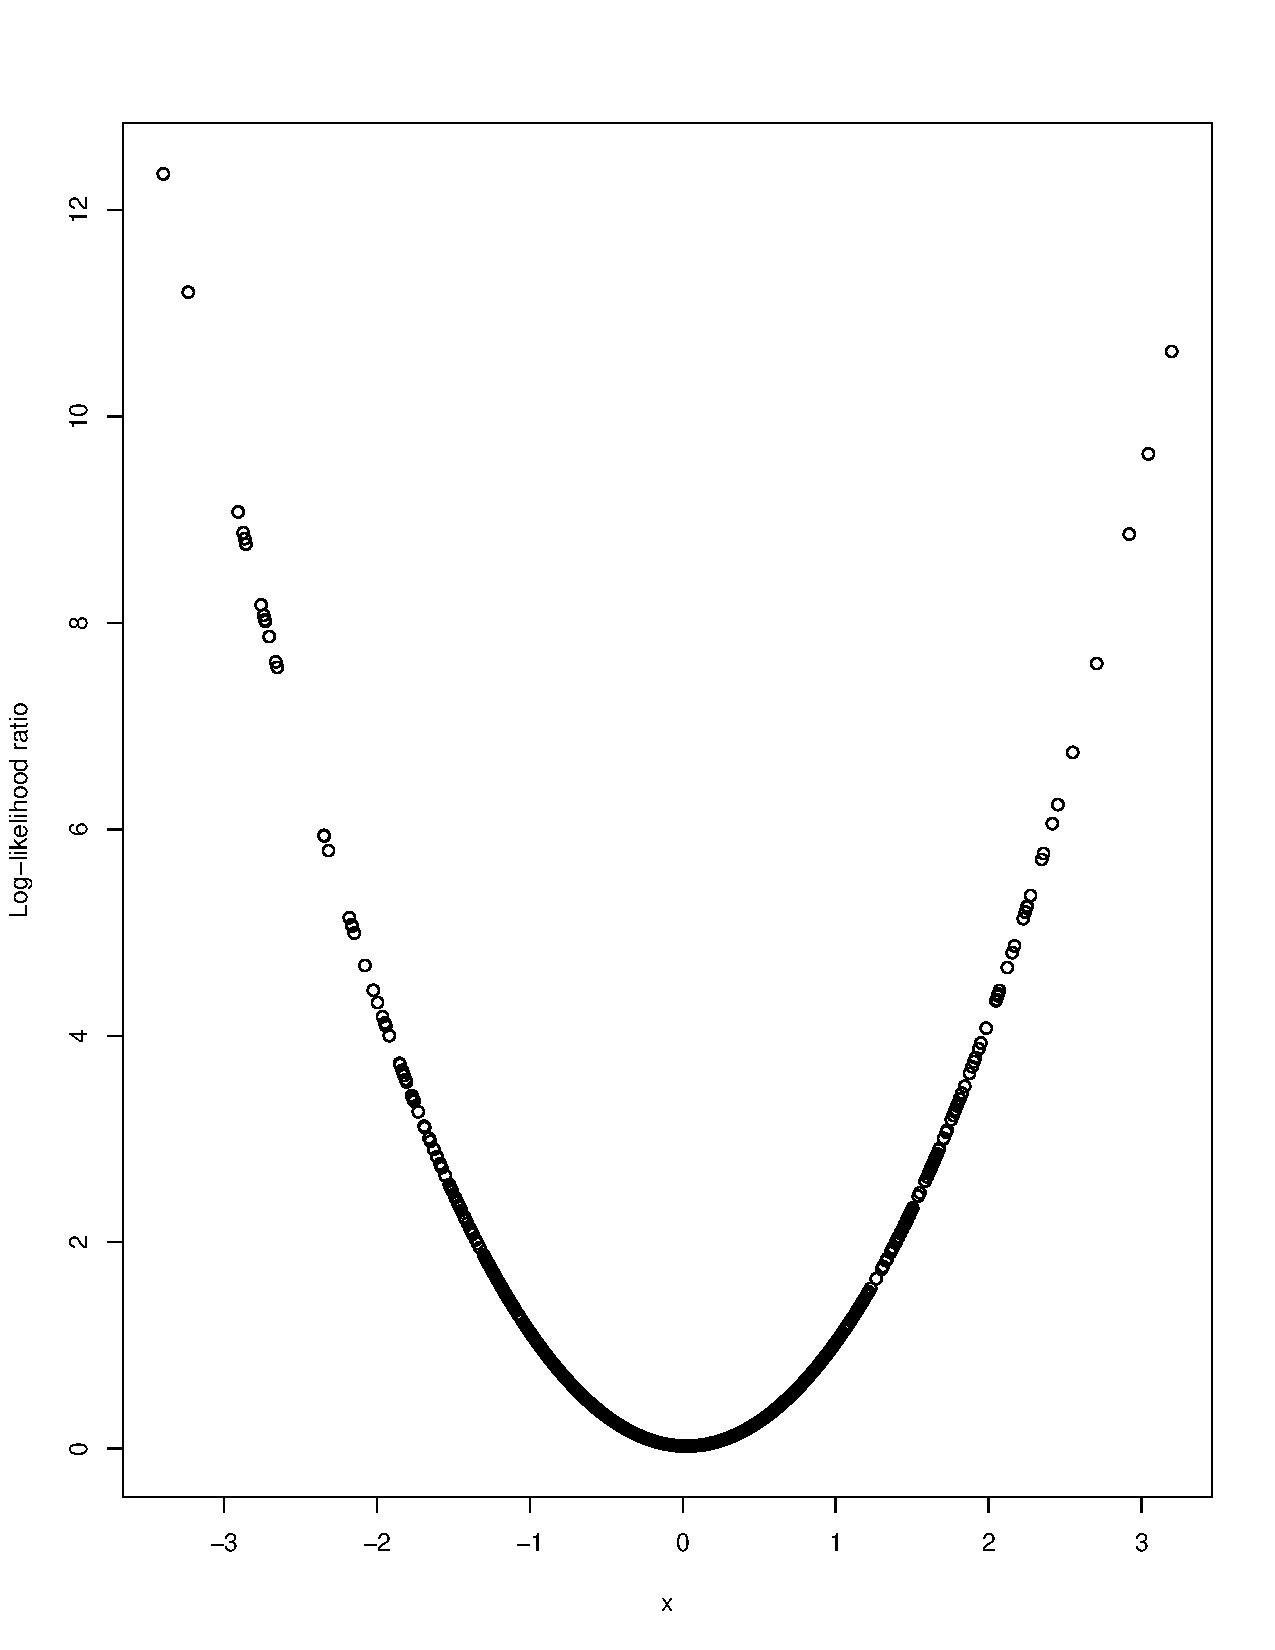
\includegraphics[scale = 0.6, height=12cm]{figures/loglik_ratio1.pdf}
    \caption{Log-likelihood ratio for $\theta = \left(0.05, 1\right)$, $\theta' = \left(0, 0.95\right)$  with $x \sim \mathcal{N}\left(0,1\right)$}
    \label{fig:loglik_ratio_gaussian}
\end{figure}
As we have seen both mathematically and graphically, it is possible to find $a$ and $b$ of the concentration bound without having to evaluate all the likelihoods. 
\subsection{Logistic model}
For a logistic regression model with parameters $\beta_0$ and $\beta_1$, the likelihood function for a single data point $y_n$ is given by 
\begin{equation}\label{eq:logist_likelihood}
\begin{split}
    L\left(\beta_0, \beta_1\right) &= p\left(x_i\right)^{y_n} \left(1 - p\left(x_n\right)\right)^{1-y_n} \\
    &= \left(\frac{1}{1 +  e^{-\beta0 -\beta_1 x_n}}\right)^{y_n} \left(1 +  \frac{1}{1 -  e^{-\beta0 -\beta_1 x_n}}\right)^{1 - y_n}. 
\end{split}
\end{equation}
Which gives the log-likelihood log-likelihood 
\begin{equation}\label{eq:logist_loglik_example}
   \ell\left(\beta_0, \beta_1\right) =   y_n\left(\beta_0 + \beta_1 x_n \right) - \log \left( 1 + e^{\beta_0  + \beta_1 x_n }\right)
   \end{equation}
Thus the log-likelihood ratio is given by 
\begin{equation}\label{eq:loglik_ratio_logistic}
\begin{split}
    \log\frac{L\left(\beta'\right)}{L\left(\beta\right)} &= \ell\left(\beta_0', \beta_1'\right) -  \ell \left(\beta_0,\beta_1\right)\\
    & = y_n\left(\beta_0' - \beta_0 + x_n \left(\beta_1' - \beta_1\right)\right) - \log \left(1 + e^{\beta_0' + \beta_1' x_n}\right) + \log \left(1 + e^{\beta_0 +  \beta_1 x_n}\right) \\
    & = y_n\left(\beta_0' - \beta_0 + x_n\left(\beta_1' - \beta_1\right)\right) + \log \left(\frac{1 + e^{\beta_0 + \beta_1 x_n}}{1 + e^{\beta_0' + \beta_1' x_n}}\right) 
    \\
    & = \begin{cases}{} 
        \log \left(\frac{1 + e^{\beta_0 + \beta_1 x_n}}{1 + \beta_0' + \beta_1' x_n}\right) & if \quad y_n = 0 \\
        \beta_0' - \beta_0 + x_n\left(\beta_1' - \beta_1\right) + \log \left(\frac{1 + e^{\beta_0 + \beta_1 x_n}}{1 + e^{\beta_0' + \beta_1'x_n}}\right)  & if \quad y_n = 1
    \end{cases}
\end{split}
\end{equation}
We plot the result of \eqref{eq:loglik_ratio_logistic} with two different values of $\theta = \left(\beta_1,\beta_2\right)$. The results are shown in figures \ref{fig:loglik_ratio_logistic} and \ref{fig:loglik_ratio_logistic2}. These log-likelihood ratios, like in the case of the normal model, seem to behave in such a way that $a$ and $b$ can be calculated without having to evaluate all the log-likelihoods. 

\begin{figure}[H]
    \centering
    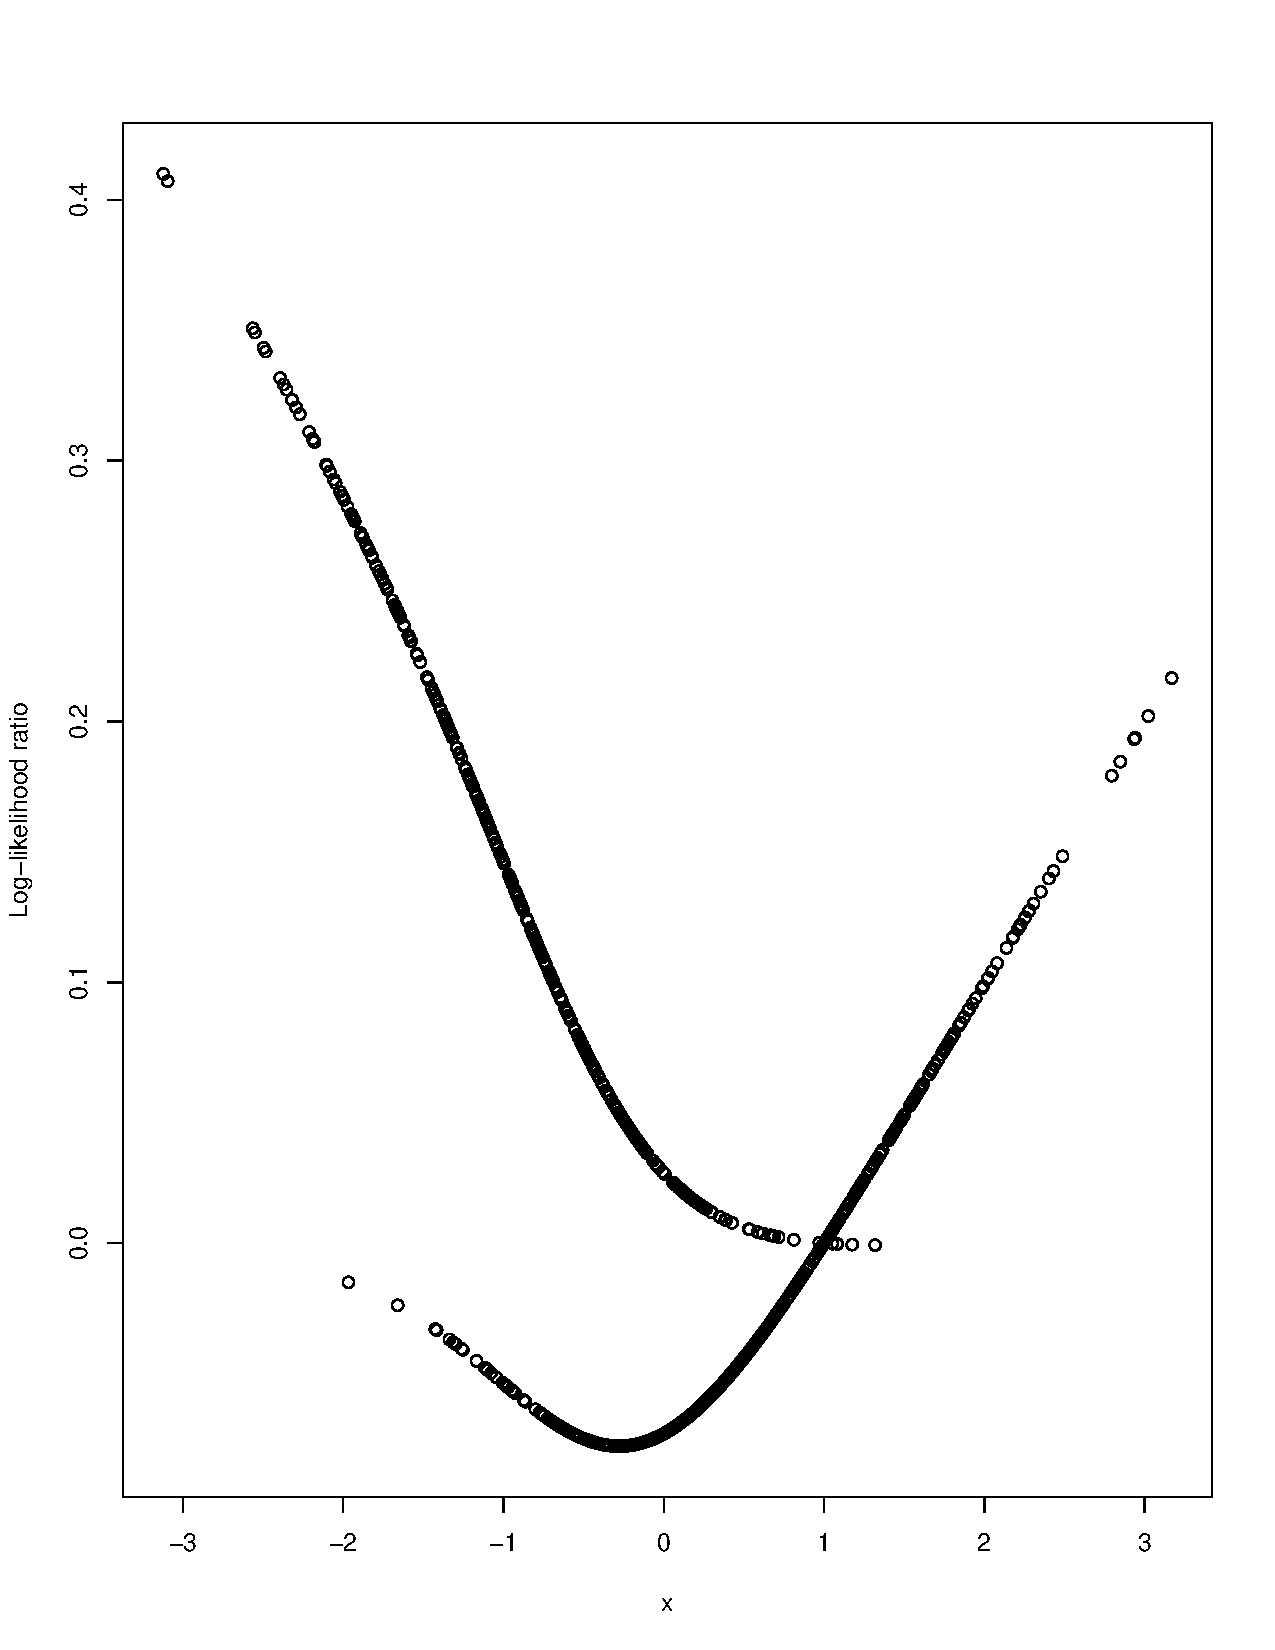
\includegraphics[scale = 0.7, height = 12cm]{figures/loglik_ratio_logistic.pdf}
    \caption{Log-likelihood ratio for $\theta = \left(\beta_0, \beta_1\right) = \left(0.95, 2.05\right), \theta' = \left(1.05, 1.95\right)$, $\theta_{True} = \left(1, 2\right)$}
    \label{fig:loglik_ratio_logistic}
\end{figure}{}
\begin{figure}
    \centering
    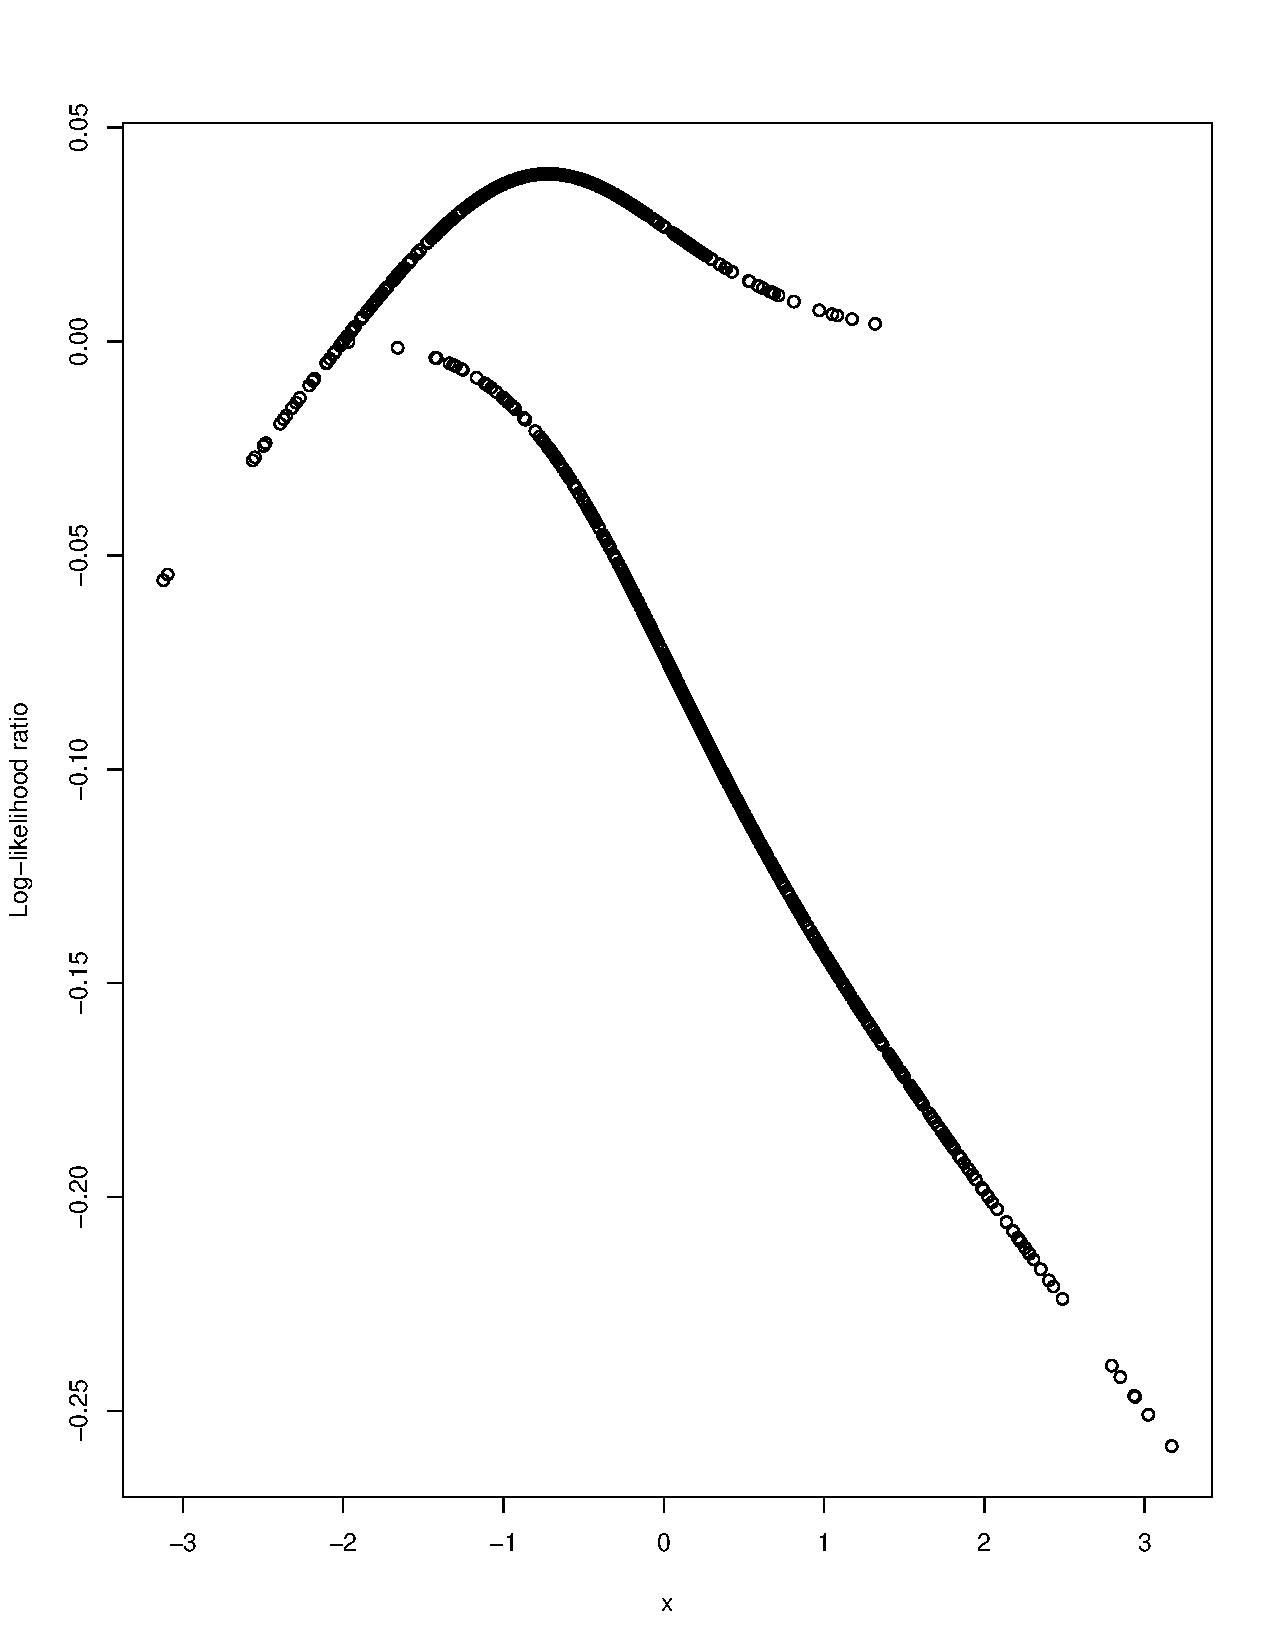
\includegraphics[scale = 0.7, height = 13cm]{figures/loglik_ratio_logist2.pdf}
    \caption{Log-likelihood ratio for $\theta = \left(\beta_0, \beta_1\right) = \left(0.95, 2.0\right), \theta' = \left(1.05, 2.2\right)$}
    \label{fig:loglik_ratio_logistic2}
\end{figure}{
A function on the form $ax + b$ is both convex and concave \todo{referanse}, while $\log\left(1 + e^x\right)$ is convex \todo{proof}. 
Thus $\log\left(\frac{1 + e^{\beta_0 + \beta_1 x}}{1 + e^{\beta_0' + \beta_1'x}}\right) = \log\left(1 + e^{\beta_0 + \beta_1}\right) - \log\left(1+ e^{ \beta_0' + \beta_1'x}\right)$ is convex if 
\begin{equation*}
\begin{split}
    \log\left(1 + e^{\beta_0 + \beta_1x}\right) &> \log\left(1 + e^{\beta_0' + \beta_1' x}\right)  \\
    \implies 1 + e^{\beta_0 + \beta_1x} &> 1 + e^{\beta_0' + \beta_1'x} \\
    \implies \beta_0 + \beta_1 x &> \beta_0' + \beta_1'x.
\end{split}{}
\end{equation*}
Similarly, the log-likelihood ratio is concave if 
\begin{equation*}
    \beta_0 + \beta_1 x < \beta_0' + \beta_1'x. 
\end{equation*}
The maximum absolute value of the log-likelihood ratio will thus be either at the extreme $x$-values or at the $x$-value closest to the global maximum or minimum for concave and convex log-likelihood ratios respectively.  To find the global maximum or minimum of the log-likelihood ratio, we have to differentiate and set equal to zero, solve for $x$, and find the $x$-value closest to the $x$-value of the global maximum/minimum. 
\section{Linear regression}
We would also like to perform linear regression using the confidence sampler. In linear regression, one assumes that the data $\mathbf{y} \sim \mathcal{N}\left(\mathbf{x}\beta, \sigma^2\right)$,
with $x$ the explanatory variables. Here, the parameter of interest $\theta = \left(\beta, \sigma\right)$    
For simple linear regression with $\beta = \left(\beta_0, \beta_1\right)$, the log-likelihood ratio is given by 
\begin{equation}
\begin{split}
    \log \frac{L\left(\theta'\right)}{L\left(\theta\right)} &= \log \frac{L\left(\beta_0', \beta_1', \sigma'\right)}{L\left(\beta_0, \beta_1, \sigma\right)}  \\
    & = \ell\left(\beta_0, \beta_1, \sigma\right) - \ell\left(\beta_0, \beta_1, \sigma\right) \\
    & = -\log\sigma' + \log\sigma - \frac{\left(y - \beta_0' - \beta_1'x\right)^2}{2\sigma'^2} + \frac{\left(y - \beta_0 - \beta_1x\right)^2}{2\sigma^2} \\
    & = \log \sigma - \log \sigma' - \frac{y^2 - 2y\beta_0'  - 2y\beta_1' + \beta_0'^2 + 2\beta_0'\beta_1'x + \beta_1'^2x^2 }{2\sigma'^2} \\ &+ \frac{y^2 - 2y\beta_0 - 2y\beta_1x + \beta_0^2 + 2\beta_0\beta_1x + \beta_1^2x^2}{2\sigma^2}
    \end{split}
\end{equation}
We plot this log-likelihood ratio as a function of $y$ to see how it behaves. The result is shown in Figure \ref{fig:loglik_ratio_linear_regression} 
\begin{figure}[H]
    \centering
    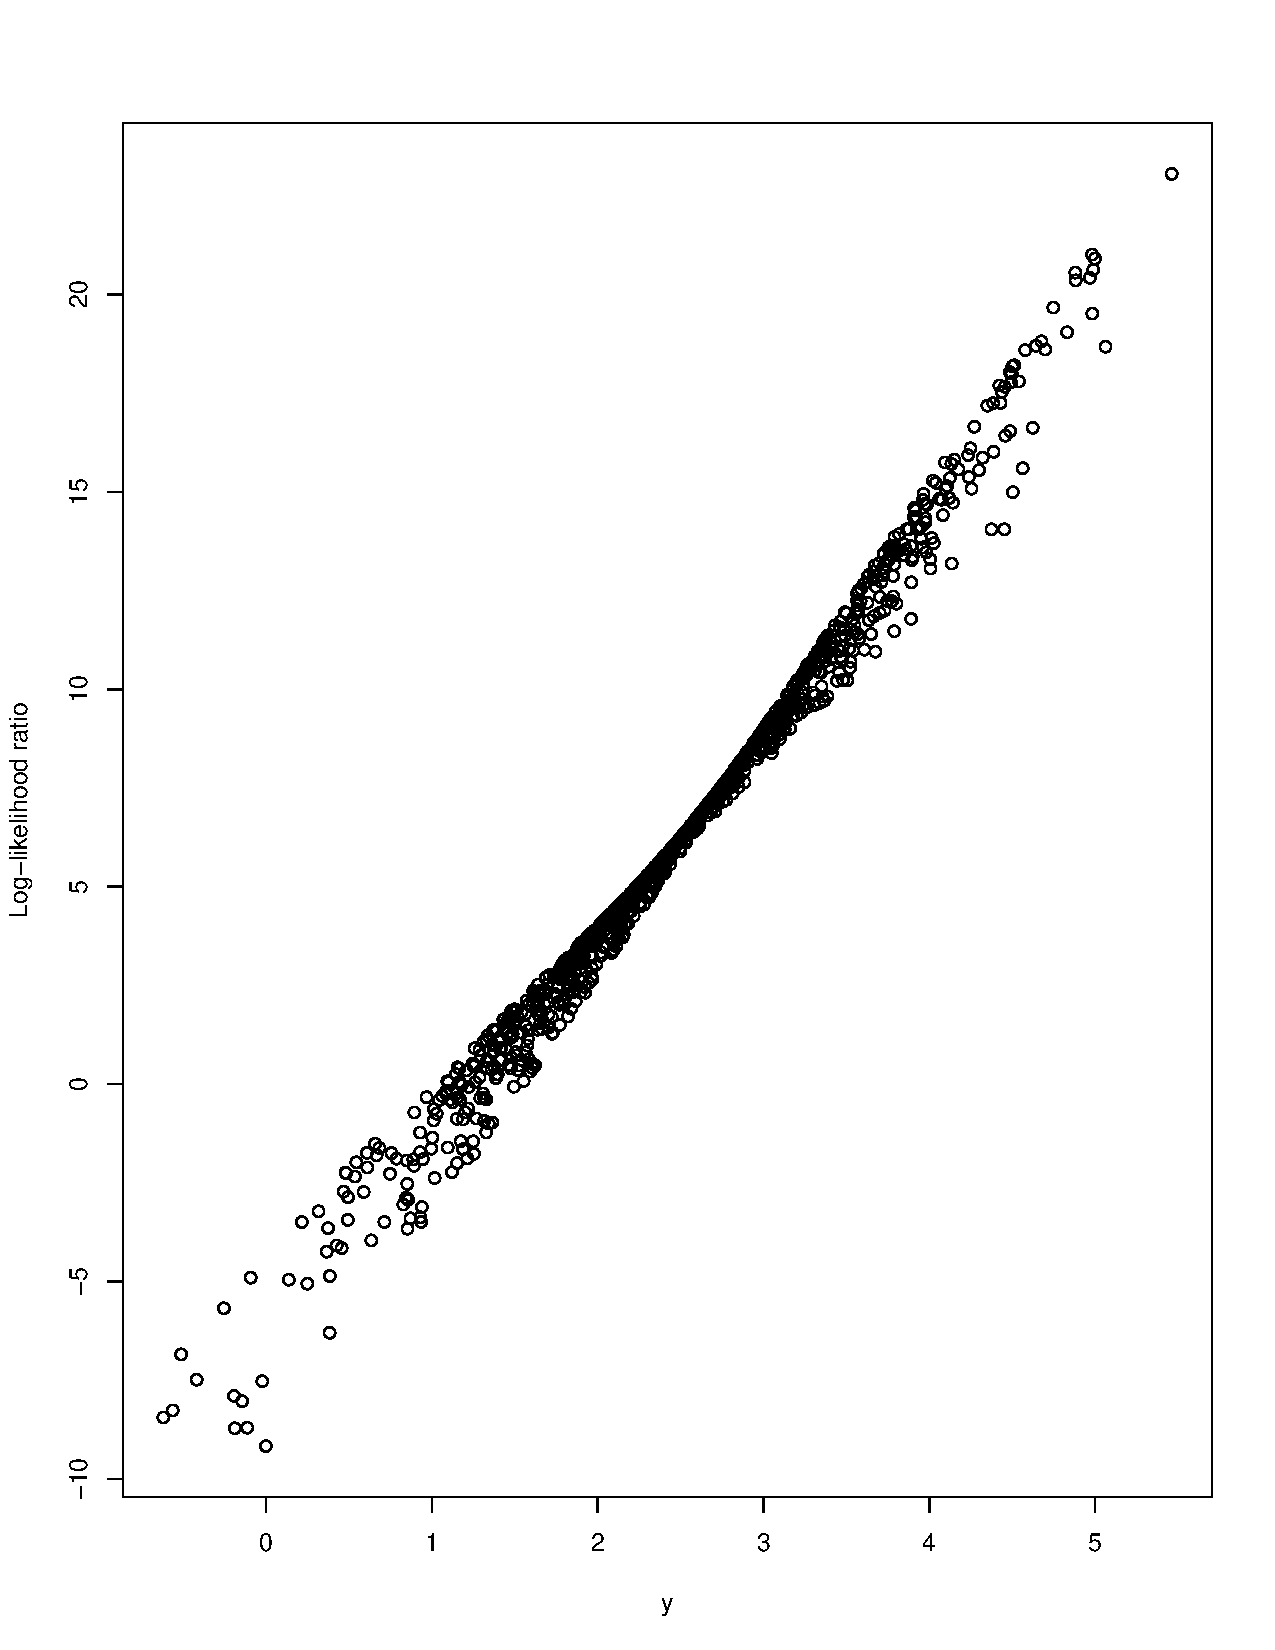
\includegraphics[scale = 0.7, height = 12cm]{figures/loglik_ratio_lin_reg.pdf}
    \caption{Log-likelihood ratio for $\theta = \left(2,1.2,  1\right), \theta' = \left(2.1, 0.9, 1.1\right), \theta_{True} = \left(2,1,1\right)$}
    \label{fig:loglik_ratio_linear_regression}
\end{figure}{}

\section{Adaptive subsampler using proxies as control variates}\label{sec:adap_subsampl}
Bardenet et al. \cite{Bardenet:1} propose using a confidence sampler with proxies for the likelihood, which act as control variates. 
Control variates are used to reduce the variance of an estimator by relating the original estimator to a known quantity. 
Say we want to estimate $EX = \theta$ with the unbiased estimator $\hat{\theta}$. Suppose we also have another random variable  $Y$ where the expectation of $Y$, $EY = \mu$ is know. 
We define $$\hat{\theta}_{CV} = \hat{\theta} + c\left(Y - \mu\right) $$  Then, $\hat{\theta}_{CV}$ will also be  an unbiased estimator of $\theta$, and if we choose $c$, correctly, it will also have a smaller variance than $\hat{\theta}$. 
This we can easily show by \begin{equation*}
\begin{split}
    \mathrm{Var}\;\hat{\theta}_{CV}  &= \mathrm{Var}\left[\hat{\theta} + c\left(Y - \mu\right)\right]
     = \mathrm{Var}\left(\hat{\theta} - cY\right) \\ & = \mathrm{Var}\;\hat{\theta} + c^2\mathrm{Var}\;Y + 2c\mathrm{Cov}\left(\hat{\theta}, Y\right)
\end{split}
\end{equation*}
We want to find the $c$ that minimizes the variance of $\hat{\theta}_{CV}$. 
\begin{equation}\label{eq:control_var}
\begin{split}
    \frac{\partial}{\partial c} \mathrm{Var}\; \hat{\theta}_{CV} &= 2c\mathrm{Var}\;Y + 2\mathrm{Cov}\left(\hat{\theta}, Y\right) = 0 \\
    & \implies c = - \frac{\mathrm{Cov}\left(\hat{\theta}, Y\right)}{\mathrm{Var}\;Y}
\end{split}
\end{equation}
We calculate the second derivative to show that the result from (\ref{eq:control_var}) is indeed a minimum
\begin{equation*}
    \frac{\partial^2}{\partial c^2} \mathrm{Var}\; \hat{\theta}_{CV}  = 2\mathrm{Var}\; Y > 0 
\end{equation*}
so $c = -\frac{\mathrm{Cov}\left(\hat{\theta}, Y\right)}{\mathrm{Var}\;Y}$ reduces the variance to a minimum. \\
The confidence sampler introduced in \cite{Bardenet:1} is an alteration of the confidence sampler in \cite{Bardenet:2}, which we described in Chapter \ref{sec:conf_sampler}. 
The bottleneck of the confidence sampler introduced in \cite{Bardenet:2} is the calculation of the expectation with respect to $\pi\left(\theta\right)q\left(\theta \mid \theta'\right)$ of the variance of the log likelihood ratio $\log \left(p\left(x\mid \theta\right)\right) / \log \left(p\left(x\mid \theta\right)\right)$ with respect to the empirical distribution of the observations.
In order to lower the variance, Bardenet et al. are inspired by Maclaurin and Adams and introduce a proxy, $\powerset\left(\theta, \theta'\right)$, defined for each data point $n$, and let the following be restrictions on $\powerset_n\left(\theta, \theta'\right)$ for any $\theta, \theta' \in \Theta$. 
\begin{enumerate}
    \item $\powerset_n\left(\theta, \theta'\right) \approx \ell_n\left(\theta'\right) - \ell_n\left(\theta\right)$
    \item $ \sum_{n = 1}^N \powerset_n\left(\theta, \theta'\right)$ can be computed cheaply
    \item $\left| \ell_n\left(\theta'\right) - \ell_n\left(\theta\right) - \powerset_i\left(\theta, \theta'\right)\right|$ can be bounded uniformly in $1\leq n \leq N$ and the bound is cheap to compute. 
\end{enumerate}
Then, the algorithm for the improved confidence sampler with proxies, is very similar to Algorithm \ref{algo:conf_sampl}, but with a few alterations:
\begin{itemize}
    \item They change Step \ref{state:lambda_star} to $\Lambda^{\star} = \frac{1}{b} \left(t \Lambda^{\star} + \sum_{n = t+1} ^b \left[ \log\frac{p\left(x_n^{\star}\mid \theta'\right)}{p\left(x_n^{\star}\mid\theta\right) } - \powerset_n\left(\theta', \theta\right) \right]\right)$.
    \item Step \ref{confidence:break_while} is replaced by $\left|\Lambda^{\star} + \frac{1}{N} \sum_{n=1}^N \powerset_n \left(\theta, \theta'\right) - \psi\left(u, \theta,\theta'\right)\right| \geq c \OR b = N$.
    \item Step \ref{confidence:accept} is replaced by $\lambda^{\star} > \psi\left(u, \theta, \theta'\right) - \frac{1}{N} \sum_{n=1}^N \powerset_n\left(\theta, \theta'\right) $. 
\end{itemize}



